\section{Design Pattern}
	I Design Pattern sono soluzioni generali a problemi ricorrenti. Il loro utilizzzo semplifica l'attivita' di progettazione, favorisce il riutilizzo del codice e rende l'architettura piu' manutenibile. Esistono diversi tipi di Design pattern e sono suddivisi in base al problema da risolvere:
	\begin{itemize}\itemsep1pt
		\item \textbf{Pattern Architetturali}: definiscono l'architettura dell'applizacione ad un livello piu' elevato rispetto ad altri Design Pattern. Esprimono schemi di base per impostare l'organizzazione di un sistema software. Si descrivono sottoinsiemi predefiniti, i ruoli che assumono e le relaioni reciproche. 
		\item \textbf{Pattern Creazionali}: permettono di nascondere i costruttori delle classi e mettono dei metodi al loro posto creando un'interfaccia. In questo modo si possono utilizzare oggetti senza sapere come sono implementati.
		\item \textbf{Pattern Strutturali}: consentono di riutilizzare degli oggetti esistenti fornendo agli utilizzatori un'interfaccia più adatta alle loro esigenze.
		\item \textbf{Pattern Comportamentali}: definiscono soluzioni per le piu' comuni interazioni tra oggetti.
	\end{itemize} 
	
	\subsection{Design Pattern Architetturali}
		\subsubsection{Microservizi}
			\begin{itemize}
				\item\textbf{Scopo dell'utilizzo}: Questo pattern è orientato ai microservizi, cioè permette di implementare unità separate distribuite;
				\item\textbf{Contesto d'utilizzo}: 
			\end{itemize}
			\begin{figure}
				\centering
				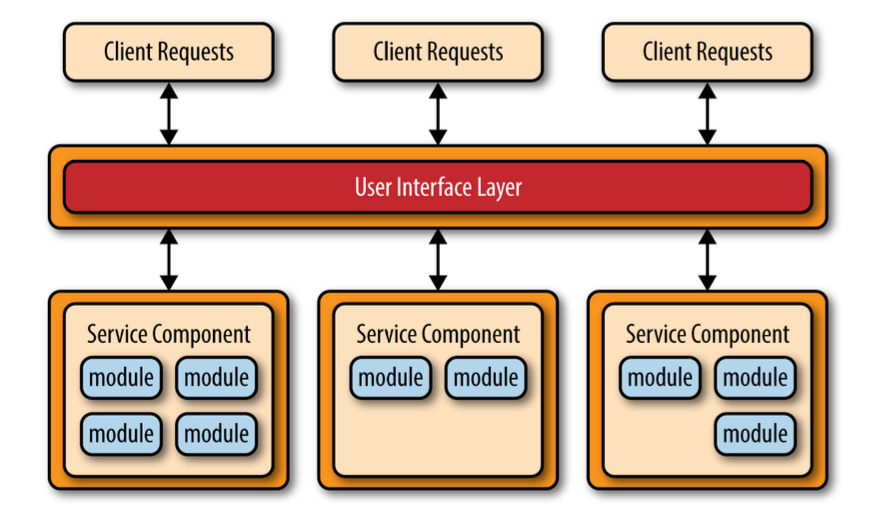
\includegraphics{ArchitetturaMicroservizi.png}
				\caption{Architettura Microservizi}
				\label{Fig. Architettura a microservizi}
			\end{figure}

		\subsubsection{Model View View Model - MVVM}
			\begin{itemize}
				\item \textbf{Scopo dell'utilizzo}: Permette di separare lo sviluppo della view dal comportamento;
				\item \textbf{Contesto d'utilizzo}: Verrà usato questo pattern per lo sviluppo del front-end. Abbiamo scelto il framework AngularJS, il quale si presta bene all'adozione della famiglia di pattern MV. L'utilizzo di questi strumenti ci permette di separare la logica di business del front-end dalla sua rappresentazione grafica.
			\end{itemize}
			\begin{figure}[h]{0.5}
				\centering
				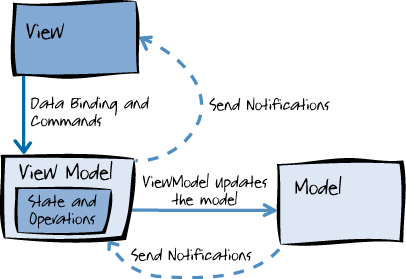
\includegraphics{mvvm.png}
				%\vspace{-40pt}
				\caption{mvvm}
				\label{fig. Mvvm}
			\end{figure}

		\subsubsection{Data Access Object - DAO }
		\begin{itemize}\itemsep1pt
				\item \textbf{Scopo dell'utilizzo}: Fornisce un'interfaccia per l'interazione con uno specifico tipo di database o in generale qualche sistema di persistenza. I vantaggi che ne derivano sono un totale disaccoppiamento tra la logica di business ed il database;
				\item \textbf{Contesto dell'utilizzo}: Questo pattern è stato scelto per la sua facilità di cooperare con Java ed i database relazionali. Crea una classe per ogni entità presente nel nostro sistema. Ognuna di questa classi conterrà poi dei metodi che le permetteranno di interagire con il database, dandole la possibilità, ad esempio, di inserire, modificare, rimuovere, aggiornare e ricercare dei dati.
		\end{itemize}
		\begin{figure}[h]{0.5}
			\centering
			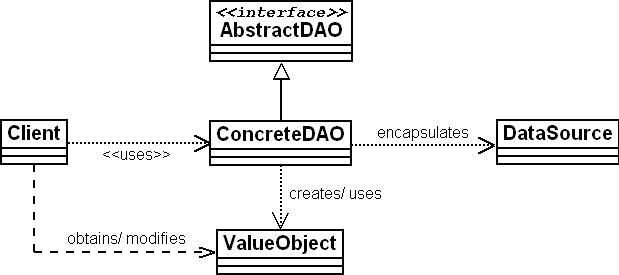
\includegraphics{dao.png }
			\caption{DAO}
			\label{fig. Data Access Object - DAO}
		\end{figure}
	\subsection{Design Pattern Creazionali}
		
		\subsubsection{Abstract Factory }
		\begin{itemize}\itemsep1pt
			\item \textbf{Scopo dell'utilizzo}: Fornisce un'interfaccia per creare famiglie di oggetti connessi o dipendenti fra loro, in modo che non ci sia necessità da parte del client di specificare i nome delle classi concrete all'interno del proprio codice;
			\item \textbf{Contesto dell'utilizzo}: Questo pattern è stato implementato per permettere di istanziare i data access object adeguati rispetto al database voluto, permettendo quindi una facile espansione futura. 
		\end{itemize}
	
		\begin{figure}[h]{0.5}
			\centering
			\incudegraphics{abstractfactory.png}
			\caption{Abstract Factory}
			\label{fig. Abstract Factory}
		\end{figure}
		
		\subsubsection{Dependency Injection}
		\begin{itemize}\itemsep1pt
			\item\textbf{Scopo dell'utilizzo}: Permette di separare il comportamento di una componente dalla risoluzione delle sue dipendenze;
			\item\textbf{Contesto dell'utilizzo}:
		\end{itemize}
	
		\begin{figure}[h]{0.5}
			\centering
			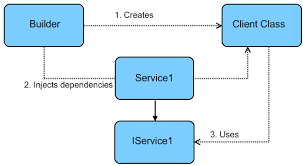
\includegraphics{DependencyInjection.png}
			\caption{Dependency Injection}
			\label{fig. Dependency Injection}
		\end{figure}

	\subsection{Design Pattern Strutturali}

		\subsubsection{Facade} 
		 \begin{itemize}
		 		\item\textbf{Scopo dell'utilizzo}: Fornisce un'interfaccia unica semplice per un sottosistema complesso, strutturando il sistema in sottoinsiemi;
		 		\item\textbf{Contesto dell'utilizzo}: 
		 \end{itemize}
	 		 	
		\begin{figure}[h]{0.5}
			\centering
			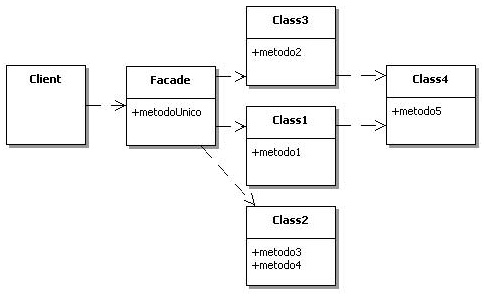
\includegraphics{facade.jpeg}
			\caption{Facade}
			\label{fig. Facade}	
		\end{figure}
		 		
	\subsection{Desgin Pattern Comportamentali} 
		
		\subsubsection{Command}
		\begin{itemize} \itemsep1pt
			\item \textbf{Scopo dell'utilizzo}: Permette di incapsulare una richiesta in un oggetto, cosicche' i client sia indipendente dalle richieste;
			\item \textbf{Contesto dell'utilizzo}: Questo pattern ci permette di facilitare il passaggio delle chiavi all'utente.
		\end{itemize}
	
		\begin{figure}[h]{0.5}
			\centering
			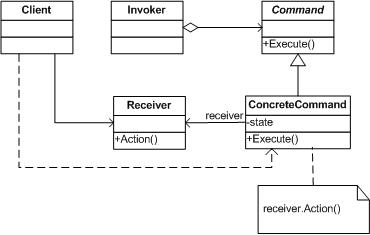
\includegraphics{command.jpeg}
			\caption{Command}
			\label{fig. Command}
		\end{figure}
			
		